\chapter{Our Voting Schemes}
\label{chap:ourVotingSchemes}

The voting schemes we use, are built from the concepts introduced in the Chapters \ref{chap:gpzkp}, \ref{chap:elGamalEncryption} and \ref{chap:ellipticCurves}.
Recall, that we introduced a voting scheme as the following seve-tuple in \cref{chap:votingschemes}:
\begin{align*}
    VS=(C, \mathcal{S}, ZPS(R_C), Setup, \{V_0, \dots, V_{n-1}, VA\})
\end{align*}
We employ \gls{eeg} based on either a Montgomery Curve or its Twisted Edwards equivalent as the encryption scheme $\mathcal{S}$.
Furthermore, we use a \gls{g16snark} as the \gls{zps} to ensure ballot validity.
To show that our approach to voting schemes can be easily adapted to many different election types, we create voting schemes based on several different choice spaces $C$.

\section{The Ballot Validity Relation $R_C$}
\label{section:ourVotingSchemes:ballotValidity}
%\todo{
%    Define complete ballot validity circuit using high-level components from the voting system in \cref{chap:votingschemes}.
%    (And note that the decomposition relation based on this circuit is equivalent to the relation $R_C$ used in \cref{chap:votingschemes}.)
%    Split into two relations $r_C^{enc}$ and $r_C^{vot}$.
%}
In \cref{chap:votingschemes}, $R_C$ is defined as the relation checking ballot validity.
Here, $R_C$ gets a ballot $b$ and auxiliary information $aux$ needed by the encryption scheme as a private witness.
The public instance is the public key $pk$ of the encryption scheme and an encrypted ballot $b'$.
As presented earlier, $R_C$ outputs $1$ if and only if two checks are fulfilled:
\begin{itemize}
    \item $b\in C$
    \item $\mathcal{S}.Enc^{aux}(b)=b'$
\end{itemize}
In order to compute a \gls{zkp} for these checks, we need to express them inside a circuit.
The algebraic function asserting $b\in C$ is called $r^{Vot}$ and the corresponding circuit is $\mathfrak{C}^{Vot}$.
How we can compute $r^{Vot}$ is highly dependent on the choice space $C$ and therefore also the election type.
Thus, we will define this in detail for the different election types in \cref{section:ourVotingSchemes:choiceSpaces}.

For the assertion $\mathcal{S}.Enc^{aux}(b)=b'$ we create an algebraic function $r^{Enc}$ and corresponding circuit $\mathfrak{C}^{Enc}$.
This function depends on the choice of the encryption scheme $\mathcal{S}$ and will be defined in \cref{section:ourVotingSchemes:encryption}.

We can combine $r^{Vot}$ and $r^{Enc}$ into the function $r^{Ballot\text{-}Validity}$ which can be computed as in \cref{alg:ballotValidity}.

\begin{Algorithmus}[h] %Use the environment only if you want to place the algorithm similar to graphics from TeX
    \caption{Function $r^{Ballot\text{-}Validity}$ used to assert Ballot validity. 
    Input is a ballot $b$, encrypted ballot $b'$, public key $pk$ and auxiliary encryption information $aux$.
    %$r^{Ballot\text{-}Validity}$ asserts $b\in C$ via $r^{Vot}$ and $\mathcal{S}.Enc^{aux}(b)=b'$ via $r^{Enc}$.
    }
    \label{alg:ballotValidity}
    \begin{algorithmic}
    \Procedure{$r^{Ballot\text{-}Validity}$}{$pk, b, aux, b'$}
        \State $r^{Vot}(b)$ \Comment Assert $b\in C$.
        \State $r^{Enc}(pk, b, aux, b')$ \Comment Assert $\mathcal{S}.Enc^{aux}(b)=b'$.
    \EndProcedure
    \end{algorithmic}
\end{Algorithmus}

The corresponding circuit $\mathfrak{C}^{Ballot\text{-}Validity}$ is presented in \cref{fig:circuit:ballotValidity}.

\begin{figure}[h]
    \centering
    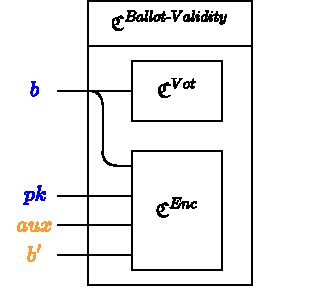
\includegraphics[scale=.8]{graphics/ourVotingSchemes/ballotValidity.pdf}
    \caption{Circuit $\mathfrak{C}^{Ballot\text{-}Validity}$, asserting Ballot Validity.
    Input is the witness consisting of a ballot $b$ and auxiliary encryption information $aux$ and the instance consisting of an encrypted ballot $b'$ and the public key $pk$.
    $\mathfrak{C}^{Ballot\text{-}Validity}$ asserts $b\in C$ via $\mathfrak{C}^{Vot}$ and $\mathcal{S}.Enc^{aux}(b)=b'$ via $\mathfrak{C}^{Enc}$.
    }
    \label{fig:circuit:ballotValidity}
\end{figure}

\section{Zero Knowledge Proof System $ZPS(R_C)$}
\label{section:ourVotingSchemes:zps}
Assume, we have a ballot validity relation $R_C$ as introduced in \cref{chap:votingschemes}.
Moreover, assume that $R_C$ is a decomposition relation $DR(QAP(R1CS(r_C)), d_p)$ for the algebraic relation $r_C$ as previously \ref{section:ourVotingSchemes:ballotValidity}.
Then, we use the \gls{g16snark} $GSNARK(R_C)=(Setup, Prove, Verify)$ based on paramters $param=(\mathbb{G}_1, \mathbb{G}_2, e(\cdot, \cdot), g_1, g_2, \mathbb{F}_q)$ as $ZPS(R_C)$.
We use the Barreto-Naehrig curve \verb|BN254| \cite{todo cite} to instantiate $\mathbb{G}_1$ and $\mathbb{G}_2$.  
This curve has the order 
\begin{align*}
    \scriptstyle q = 21888242871839275222246405745257275088548364400416034343698204186575808495617
\end{align*}
which is used to define $\mathbb{F}_q$.
Therefore, $R_C$ operates over elements of $\mathbb{F}_q$.
For the bilinear pairing $e(\cdot, \cdot)$, we choose the Weil pairing or a variant of this. \cite{huber_zk-snarks_2025}

\section{Encryption Scheme $\mathcal{S}$}
\label{section:ourVotingSchemes:encryption}
We use an \gls{eeg} scheme $\mathcal{S}=(Gen(1^\eta), Enc, Dec)$ because it is homomorphic and therefore allows us to aggregate ballots in their encrypted form. \cref{chap:elGamalEncryption}
Furthermore, we choose an elliptic curve as the group $\mathbb{G}$ that $\mathcal{S}$ is based on for security reasons. \cref{chap:ellipticCurves}

As established in \cref{section:ourVotingSchemes:zps}, our $GSNARK(R_C)$ requires that $R_C$ operates over $\mathbb{F}_q$ with 
\begin{align*}
    \scriptstyle q = 21888242871839275222246405745257275088548364400416034343698204186575808495617\text{.}
\end{align*}
Therefore, as the elliptic curve $\mathbb{G}$ used in $\mathcal{S}$, we need to choose one that operates over elements of $\mathbb{F}_q$.
Here, we implement two options: 
Either, we use the Montgomery Curve $M_{126932, 1}(\mathbb{F}_q)$ or the isomorphic Twisted Edwards Curve $TE_{126934, 126930}(\mathbb{F}_q)$.
Huber et. al. \cite{huber_zk-snarks_2025} used the Montgomery Curve in their implementation.
However, as discussed in \cref{chap:ellipticCurves}, Twisted Edwards Curves can offer more efficient group exponentiation if we provide a list of powers of the element to exponentiate.

\todo{
    Define Encryption Circuit sepearately for Twisted Edwards and Montgomery Curves.
    Maybe put powers of $g$ and $pk$ into the public key in a slightly modified version of \gls{eeg} (Define this in ElGamal chapter \ref{chap:elGamalEncryption}).
    Based on this, define $\mathfrak{C}^{Enc}$.
    Mention that encryption is done componentwise and therefore onyl dependent on the dimensions of the choice space but not its actual definition.
}


\section{Choice Spaces $C$}
\label{section:ourVotingSchemes:choiceSpaces}
The choice space $C$ in a voting system $VS$ only influences the relation $R_C$ and by extension the \gls{zps} instantiation but not any other part of the voting scheme.
As described in \cref{section:ourVotingSchemes:ballotValidity}, there is an algebraic function $r_C$ and a function $d_p$ for which $R_C=DR(QAP(R1CS(r_C)), d_p)$.
Here, $r_C$ can be split into a part $r_C^{Enc}$ for ensuring correct encryption and a part $r_C^{Vot}$ for ensuring that a ballot $b$ is part of $C$.
Since encryption is done component-wise, $r_C^{Enc}$ is only influenced by the dimensions of $C$.
Therefore, to instantiate our voting scheme $VS$ with a new election type, we only need to define the choice space $C$ and the corresponding algebraic function $r_C^{Vot}$ for this election type.

As in \cite{huber_zk-snarks_2025}, we cover a variety of election types ranging from simple Single-Vote to more complicated ranking-based types like Condorcet.


\subsection{Single-Vote}
In a Single-Vote election, a voter can choose from a fixed set of candidates. 
Here, each voter can vote for at most one of the candidates.
Therefore, it is also possible to abstain from the vote.
The example voting system introduced in \cref{chap:votingschemes} is election of this type.

\begin{definition}[Single-Vote System]
    Let $m\in\mathbb{N}$ be the number of candidates, let $\mathbb{F}_q$ be a field.
    Then, the corresponding Single-Vote choice space is defined as follows:
    \begin{align*}
        C_{\text{Single}, m}=\left\{(b_0,\dots, b_{m-1})|\forall i\in\{0,\dots, m-1\}: b_i\in\{0,1\}\:\land\: \sum_{i=0}^{m-1}b_i\in\{0,1\}\right\}
    \end{align*}
    The relation $r_{\text{Single}, m}^{Vot}:\mathbb{F}_q^m\to\emptyset$ asserts that a given ballot $b\in\mathbb{F}_q^{m}$ is in the choice space.
    To do so, the function asserts that all individual entries of $b$ are a bit and that the sum of all entries is a bit.
    Formally, let $b=(b_0,\dots, b_{m-1})\in\mathbb{F}_q^m$. Then, $r_{\text{Single}, m}^{Vot}$ operates as shown in \cref{alg:singleVoteVoting}.

    Here, the corresponding circuit $\mathfrak{C}_{\text{Single},m}^{Vot}$ is satisfied by a ballot $b=(b_0,\dots, b_{m-1})\in\mathbb{F}_q^m$ if and only if $b\in C_{\text{Single}, m}$.
    We can represent this circuit graphically as in \cref{fig:circuit:singleVoteVoting}.

    The voting system based on the choice space $C_{\text{Singe}, m}$ is $VS_{\text{Single}, m}$.
\end{definition}

\begin{Algorithmus}[h] %Use the environment only if you want to place the algorithm similar to graphics from TeX
    \caption{Function $r_{\text{Single}, m}^{Vot}$ used to assert that a ballot $b$ is part of the choice space $C_{\text{Single, m}}$.}
    \label{alg:singleVoteVoting}
    \begin{algorithmic}
    \Procedure{$r_{\text{Single}, m}^{Vot}$}{$b$}
        \State $(b_0,\dots, b_{m-1}):=b$
        \State $sum\gets 0$
        \For{$i\in\{0,\dots, m-1\}$}
            \State $r_{assert\text{-}Bit}(b_i)$
            \State $sum \gets sum + b_i$
        \EndFor
        \State $r_{assert\text{-}Bit}(sum)$
    \EndProcedure
    \end{algorithmic}
\end{Algorithmus}

\begin{figure}[h]
    \centering
    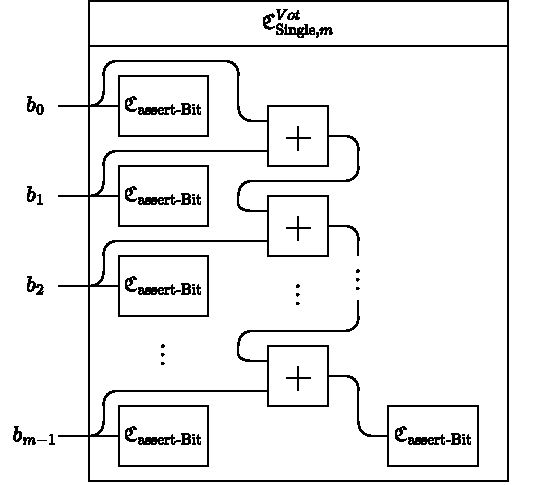
\includegraphics[scale=.8]{graphics/ourVotingSchemes/singleVoteVoting.pdf}
    \caption{Circuit $\mathfrak{C}_{\text{Single}, m}^{Vot}$, asserting that a ballot $b$ is part of the choice space $C_{\text{Single, m}}$.}
    \label{fig:circuit:singleVoteVoting}
\end{figure}

Note that $\mathfrak{C}_{\text{Single}, 3}^{Vot}$ is equivalent to $\mathfrak{C}_{assert\text{-}3\text{-}vot}$ in \cref{fig:circuit:threeVotModularity}.



\subsection{Multi-Vote}

\subsubsection{Line-Vote}

\subsubsection{\gls{mwr}}


\subsection{Borda Elections}

\subsubsection{Pointlist-Borda}

\subsubsection{\gls{bts}}


\subsection{Condorcet Methods}


\subsection{Majority Judgment}


